% Options for packages loaded elsewhere
\PassOptionsToPackage{unicode}{hyperref}
\PassOptionsToPackage{hyphens}{url}
%
\documentclass[
  ignorenonframetext,
]{beamer}
\usepackage{pgfpages}
\setbeamertemplate{caption}[numbered]
\setbeamertemplate{caption label separator}{: }
\setbeamercolor{caption name}{fg=normal text.fg}
\beamertemplatenavigationsymbolsempty
% Prevent slide breaks in the middle of a paragraph
\widowpenalties 1 10000
\raggedbottom
\setbeamertemplate{part page}{
  \centering
  \begin{beamercolorbox}[sep=16pt,center]{part title}
    \usebeamerfont{part title}\insertpart\par
  \end{beamercolorbox}
}
\setbeamertemplate{section page}{
  \centering
  \begin{beamercolorbox}[sep=12pt,center]{part title}
    \usebeamerfont{section title}\insertsection\par
  \end{beamercolorbox}
}
\setbeamertemplate{subsection page}{
  \centering
  \begin{beamercolorbox}[sep=8pt,center]{part title}
    \usebeamerfont{subsection title}\insertsubsection\par
  \end{beamercolorbox}
}
\AtBeginPart{
  \frame{\partpage}
}
\AtBeginSection{
  \ifbibliography
  \else
    \frame{\sectionpage}
  \fi
}
\AtBeginSubsection{
  \frame{\subsectionpage}
}
\usepackage{lmodern}
\usepackage{amssymb,amsmath}
\usepackage{ifxetex,ifluatex}
\usepackage{multicol}
\ifnum 0\ifxetex 1\fi\ifluatex 1\fi=0 % if pdftex
  \usepackage[T1]{fontenc}
  \usepackage[utf8]{inputenc}
  \usepackage{textcomp} % provide euro and other symbols
\else % if luatex or xetex
  \usepackage{unicode-math}
  \defaultfontfeatures{Scale=MatchLowercase}
  \defaultfontfeatures[\rmfamily]{Ligatures=TeX,Scale=1}
\fi
\usetheme[]{CambridgeUS}
\usefonttheme{structurebold}
% Use upquote if available, for straight quotes in verbatim environments
\IfFileExists{upquote.sty}{\usepackage{upquote}}{}
\IfFileExists{microtype.sty}{% use microtype if available
  \usepackage[]{microtype}
  \UseMicrotypeSet[protrusion]{basicmath} % disable protrusion for tt fonts
}{}
\makeatletter
\@ifundefined{KOMAClassName}{% if non-KOMA class
  \IfFileExists{parskip.sty}{%
    \usepackage{parskip}
  }{% else
    \setlength{\parindent}{0pt}
    \setlength{\parskip}{6pt plus 2pt minus 1pt}}
}{% if KOMA class
  \KOMAoptions{parskip=half}}
\makeatother
\usepackage{xcolor}
\IfFileExists{xurl.sty}{\usepackage{xurl}}{} % add URL line breaks if available
\IfFileExists{bookmark.sty}{\usepackage{bookmark}}{\usepackage{hyperref}}
\hypersetup{
  pdftitle={LearnR, ThinkR, and UseR},
  hidelinks,
  pdfcreator={LaTeX via pandoc}}
\urlstyle{same} % disable monospaced font for URLs
\newif\ifbibliography
\usepackage{color}
\usepackage{fancyvrb}
\newcommand{\VerbBar}{|}
\newcommand{\VERB}{\Verb[commandchars=\\\{\}]}
\DefineVerbatimEnvironment{Highlighting}{Verbatim}{commandchars=\\\{\}}
% Add ',fontsize=\small' for more characters per line
\usepackage{framed}
\definecolor{shadecolor}{RGB}{248,248,248}
\newenvironment{Shaded}{\begin{snugshade}}{\end{snugshade}}
\newcommand{\AlertTok}[1]{\textcolor[rgb]{0.94,0.16,0.16}{#1}}
\newcommand{\AnnotationTok}[1]{\textcolor[rgb]{0.56,0.35,0.01}{\textbf{\textit{#1}}}}
\newcommand{\AttributeTok}[1]{\textcolor[rgb]{0.77,0.63,0.00}{#1}}
\newcommand{\BaseNTok}[1]{\textcolor[rgb]{0.00,0.00,0.81}{#1}}
\newcommand{\BuiltInTok}[1]{#1}
\newcommand{\CharTok}[1]{\textcolor[rgb]{0.31,0.60,0.02}{#1}}
\newcommand{\CommentTok}[1]{\textcolor[rgb]{0.56,0.35,0.01}{\textit{#1}}}
\newcommand{\CommentVarTok}[1]{\textcolor[rgb]{0.56,0.35,0.01}{\textbf{\textit{#1}}}}
\newcommand{\ConstantTok}[1]{\textcolor[rgb]{0.00,0.00,0.00}{#1}}
\newcommand{\ControlFlowTok}[1]{\textcolor[rgb]{0.13,0.29,0.53}{\textbf{#1}}}
\newcommand{\DataTypeTok}[1]{\textcolor[rgb]{0.13,0.29,0.53}{#1}}
\newcommand{\DecValTok}[1]{\textcolor[rgb]{0.00,0.00,0.81}{#1}}
\newcommand{\DocumentationTok}[1]{\textcolor[rgb]{0.56,0.35,0.01}{\textbf{\textit{#1}}}}
\newcommand{\ErrorTok}[1]{\textcolor[rgb]{0.64,0.00,0.00}{\textbf{#1}}}
\newcommand{\ExtensionTok}[1]{#1}
\newcommand{\FloatTok}[1]{\textcolor[rgb]{0.00,0.00,0.81}{#1}}
\newcommand{\FunctionTok}[1]{\textcolor[rgb]{0.00,0.00,0.00}{#1}}
\newcommand{\ImportTok}[1]{#1}
\newcommand{\InformationTok}[1]{\textcolor[rgb]{0.56,0.35,0.01}{\textbf{\textit{#1}}}}
\newcommand{\KeywordTok}[1]{\textcolor[rgb]{0.13,0.29,0.53}{\textbf{#1}}}
\newcommand{\NormalTok}[1]{#1}
\newcommand{\OperatorTok}[1]{\textcolor[rgb]{0.81,0.36,0.00}{\textbf{#1}}}
\newcommand{\OtherTok}[1]{\textcolor[rgb]{0.56,0.35,0.01}{#1}}
\newcommand{\PreprocessorTok}[1]{\textcolor[rgb]{0.56,0.35,0.01}{\textit{#1}}}
\newcommand{\RegionMarkerTok}[1]{#1}
\newcommand{\SpecialCharTok}[1]{\textcolor[rgb]{0.00,0.00,0.00}{#1}}
\newcommand{\SpecialStringTok}[1]{\textcolor[rgb]{0.31,0.60,0.02}{#1}}
\newcommand{\StringTok}[1]{\textcolor[rgb]{0.31,0.60,0.02}{#1}}
\newcommand{\VariableTok}[1]{\textcolor[rgb]{0.00,0.00,0.00}{#1}}
\newcommand{\VerbatimStringTok}[1]{\textcolor[rgb]{0.31,0.60,0.02}{#1}}
\newcommand{\WarningTok}[1]{\textcolor[rgb]{0.56,0.35,0.01}{\textbf{\textit{#1}}}}
\usepackage{graphicx,grffile}
\makeatletter
\def\maxwidth{\ifdim\Gin@nat@width>\linewidth\linewidth\else\Gin@nat@width\fi}
\def\maxheight{\ifdim\Gin@nat@height>\textheight\textheight\else\Gin@nat@height\fi}
\makeatother
% Scale images if necessary, so that they will not overflow the page
% margins by default, and it is still possible to overwrite the defaults
% using explicit options in \includegraphics[width, height, ...]{}
\setkeys{Gin}{width=\maxwidth,height=\maxheight,keepaspectratio}
% Set default figure placement to htbp
\makeatletter
\def\fps@figure{htbp}
\makeatother
\setlength{\emergencystretch}{3em} % prevent overfull lines
\providecommand{\tightlist}{%
  \setlength{\itemsep}{0pt}\setlength{\parskip}{0pt}}
\setcounter{secnumdepth}{-\maxdimen} % remove section numbering

\title{RStudio, R packages, and R project}
\subtitle{A typical data science workflow in R}
\date{September 28, 2019}
\titlegraphic{\hspace*{8.5cm}
\includegraphics[width=7cm, height=2cm]{Images/Logo.JPG}}

\begin{document}
\frame{\titlepage}


\begin{frame}{About Me}
\protect\hypertarget{about-me}{}
\pause

\textbf{Name}: Ezekiel Adebayo Ogundepo \pause

\textbf{Twitter}: \href{https://twitter.com/gbganalyst}{@gbganalyst}
\pause

\textbf{GitHub}: \url{www.github.com/gbganalyst} \pause

\textbf{Website}: \url{https://bit.ly/gbganalyst}

\end{frame}

\begin{frame}{Table of contents}
	\tableofcontents[hideallsubsections]
\end{frame}

\begin{frame}

\begin{center}
\textbf{Relax, programming in R is cool!}
\end{center}
\pause
If you doubt me, please ask \pause

\begin{multicols}{3}
\textbf{Hadley Wickham}: 
\includegraphics[height=3cm, width=5cm]{Images/Hadley.JPG}

\pause
\textbf{Jenny Bryan}: 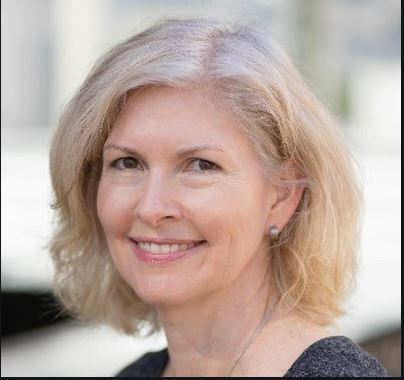
\includegraphics[height=3cm, width=5cm]{Images/Jenny.JPG} \pause

\textbf{Adeyinka
Oresanya}: 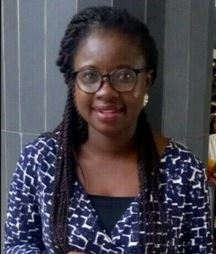
\includegraphics[height=4cm, width=5cm]{Images/Oresanya.JPG}

\end{multicols}
\end{frame}

\section{R and RStudio}
\begin{frame}{What is R programming?}
\protect\hypertarget{what-is-r-programming}{}
\pause
R is a statistical programming language for data cleaning, analysis, and visualization \pause

\begin{figure}
\centering
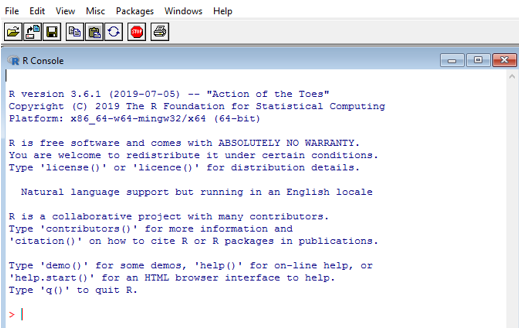
\includegraphics[height=5.8cm, width=13cm]{Images/R.png}
\caption{R programming}
\end{figure}

\end{frame}

\begin{frame}{What about RStudio?}
\protect\hypertarget{what-about-rstudio}{}
\pause
R Studio is an integrated development environment (IDE) for R
programming. R Studio makes programming easier and friendly in R.

\end{frame}

\begin{frame}{R studio}
\protect\hypertarget{r-studio}{}

\begin{figure}
\centering
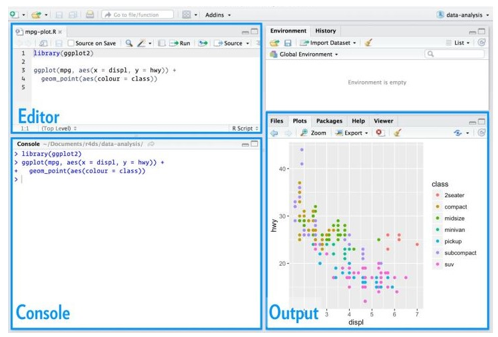
\includegraphics[height=7cm, width= 12cm]{Images/R_studio.PNG}
\caption{R studio}
\end{figure}

\end{frame}

\begin{frame}[fragile]{R packages and library}
\protect\hypertarget{r-packages-and-library}{}

A package is a collection of R functions that extends basic R
functionality (base::functions). \pause

A package can contain a set of functions relating to a specific topic or
tasks. For example, data wrangling packages include tidyr, janitor, etc.
\pause

The location where the packages are stored is called the library. If there is a particular package that you need, you can install the package from the Comprehensive R Achieve Network (CRAN) by using:\pause

\begin{Shaded}
\begin{Highlighting}[]
\KeywordTok{install.packages}\NormalTok{(}\StringTok{"pkg_name"}\NormalTok{)}
\end{Highlighting}
\end{Shaded}

\end{frame}
\section{R packages and library}
\begin{frame}[fragile]{R packages and library}
\protect\hypertarget{r-packages-and-library-1}{}
\pause
Other packages that are not yet on CRAN can also be installed from
GitHub by using devtools package e.g.~fakir \pause

\begin{Shaded}
\begin{Highlighting}[]
\KeywordTok{library}\NormalTok{(devtools)}
\KeywordTok{install_github}\NormalTok{(}\StringTok{"ThinkR-open/fakir"}\NormalTok{)}
\end{Highlighting}
\end{Shaded}

\end{frame}

\begin{frame}[fragile]{Import or load a package}
\protect\hypertarget{import-or-load-a-package}{}

\pause
To actually use the package, you need to use the command
\pause
\begin{Shaded}
\begin{Highlighting}[]
\KeywordTok{library}\NormalTok{(}\StringTok{"pkg_name"}\NormalTok{)}
\end{Highlighting}
\end{Shaded}
\pause
which makes that package functions available to you at the R session.

\end{frame}

\begin{frame}[fragile]{Library}
\protect\hypertarget{library}{}
\pause
Library is a directory where the packages are stored. You can have
multiple libraries on your hard disk. \pause

To see which libraries are available (which paths are searched for
packages): \pause

\begin{Shaded}
\begin{Highlighting}[]
\KeywordTok{.libPaths}\NormalTok{()}
\end{Highlighting}
\end{Shaded}

\begin{verbatim}
## [1] "C:/Users/OGUNDEPO EZEKIEL .A/Documents/R/win-library/3.6"
## [2] "C:/Program Files/R/R-3.6.1/library"
\end{verbatim}

\end{frame}

\begin{frame}[fragile]{}
\protect\hypertarget{section}{}
And to see which packages are there: \pause
\begin{Shaded}
\begin{Highlighting}[]
\KeywordTok{lapply}\NormalTok{(}\KeywordTok{.libPaths}\NormalTok{(), dir)}
\end{Highlighting}
\end{Shaded}

\begin{verbatim}
## [[1]]
##   [1] "abind"             "acepack"           "ada"              
##   [4] "askpass"           "assertthat"        "attempt"          
##   [7] "AUC"               "babynames"         "backports"        
##  [10] "bartMachine"       "bartMachineJARs"   "base64enc"        
##  [13] "BBmisc"            "BH"                "bibtex"           
##  [16] "bit"               "bit64"             "bitops"           
##  [19] "blob"              "blogdown"          "bookdown"         
##  [22] "brew"              "broom"             "BSDA"             
##  [25] "bst"               "C50"               "callr"            
##  [28] "car"               "carData"           "caret"            
##  [31] "catboost"          "caTools"           "cellranger"       
##  [34] "charlatan"         "checkmate"         "citr"             
##  [37] "classInt"          "cli"               "clipr"            
##  [40] "clisymbols"        "coin"              "colorspace"       
##  [43] "combinat"          "commonmark"        "config"           
\end{verbatim}

\end{frame}

\begin{frame}[fragile]{\texttt{library(x)} or \texttt{require(x)}?}
\protect\hypertarget{libraryx-or-requirex}{}
\pause
\texttt{library(package)} and \texttt{require(package)} both load the
namespace of the package with name package and attach it on the search
list. require is designed for use inside other functions; it returns
FALSE and gives a warning (rather than an error as \texttt{library()}
does by default) if the package does not exist.

\end{frame}

\begin{frame}[fragile]{Remove installed packages}
\protect\hypertarget{remove-installed-packages}{}
\pause
Removes installed packages/bundles and updates index information as
necessary.

\begin{Shaded}
\begin{Highlighting}[]
\KeywordTok{remove.packages}\NormalTok{(}\StringTok{"pkg_name"}\NormalTok{)}
\end{Highlighting}
\end{Shaded}

\end{frame}

\begin{frame}[fragile]{Using functions in other packages with Double
Colon operator}
\protect\hypertarget{using-functions-in-other-packages-with-double-colon-operator}{}
\pause
There are many ways to make use of functions in other packages. You can
load the package with \texttt{library(pkg\_name)} and then just use the
functions. Or you can use the :: operator, for example writing
\texttt{janitor::clean\_name()} rather than \texttt{library(janitor)}
and then \texttt{clean\_name()}. \pause

The move is towards the latter, where only the necessary functions will
be loaded, rather than attaching the whole package. So to carry the
reader of your article on which function belongs to a particular
package, it is better to use \texttt{package\_name::function()}

\end{frame}
\section{RStudio project}

\begin{frame}[fragile]{Where Does Your Analysis Live?}
\protect\hypertarget{where-does-your-analysis-live}{}
\pause
The working directory is where R looks for files that you ask it to
load, and where it will put any files that you ask it to save.\pause

RStudio shows your current working directory at the top of the console:

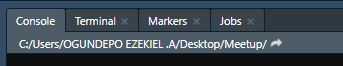
\includegraphics{Images/wd.JPG} \pause

And you can also print this out by using:

\begin{Shaded}
\begin{Highlighting}[]
\KeywordTok{getwd}\NormalTok{()}
\end{Highlighting}
\end{Shaded}

\begin{verbatim}
## [1] "C:/Users/OGUNDEPO EZEKIEL .A/Desktop/Meetup"
\end{verbatim}

\end{frame}

\begin{frame}[fragile]{}
\protect\hypertarget{section-1}{}

If you have specific directory and you want to use that as your working
directory, in R you can do that with the command \texttt{setwd()} e.g. \pause

\begin{Shaded}
\begin{Highlighting}[]
\KeywordTok{setwd}\NormalTok{(}\StringTok{"/path/to/my/data_analysis"}\NormalTok{)}
\end{Highlighting}
\end{Shaded}

or by using the keyboard shortcut with \texttt{Ctrl+Shift+H} and choose
that specific directory (Folder).

\end{frame}

\begin{frame}[fragile]{Paths and Directories}
\protect\hypertarget{paths-and-directories}{}
\pause
\begin{itemize}
\tightlist
\item
  Absolute paths: This looks different in every computer. In Windows
  they start with a drive letter (e.g., C:). In my R working directory I
  have \texttt{"C:/Users/OGUNDEPO\ EZEKIEL.A/Desktop/Meetup"} as
  absolute path.
\end{itemize}
\pause
You should never use absolute paths in your scripts, because they hinder
sharing and no one else will have exactly the same directory
configuration as you.
\pause
\begin{itemize}
\tightlist
\item
  Relative paths: With the help of library \texttt{here::here()} or
  \texttt{R\ project} we can have a relative path like
  \texttt{data/submission\_format.csv} that allow for file sharing and
  collaboration.
\end{itemize}

\end{frame}

\begin{frame}{RStudio Projects}
\protect\hypertarget{rstudio-projects}{}
\pause
For a typical data science workflow, you should use Rstudio project.

R experts keep all the files associated with a project together---like
data folder, R scripts folder, analytical results folder, figures
folder. This is such a wise and common practice.

\end{frame}

\begin{frame}{}
\protect\hypertarget{section-2}{}

\begin{figure}
\centering
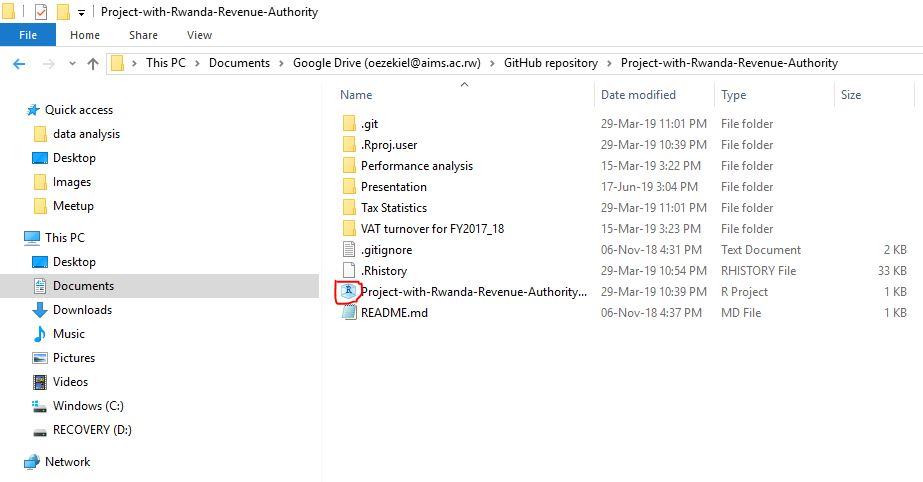
\includegraphics{Images/R project.JPG}
\caption{Example of Rstudio project}
\end{figure}

\end{frame}


\begin{frame}{Creating a new R project}
\pause
Click File → New Project, then choose Existing Directory:
\begin{figure}
	\centering
	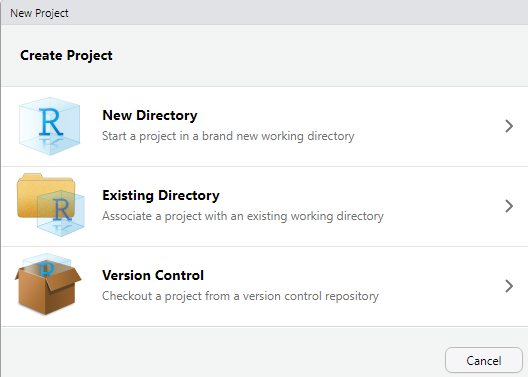
\includegraphics[height=7cm, width= 12cm]{Images/step1.PNG}
\end{figure}
\end{frame}

\begin{frame}{}
\protect\hypertarget{section-3}{}

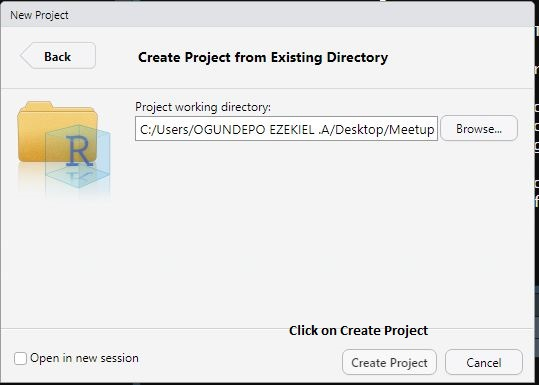
\includegraphics{Images/step2.JPG}

\end{frame}

\begin{frame}{}
\protect\hypertarget{section-4}{}

\begin{figure}
\centering
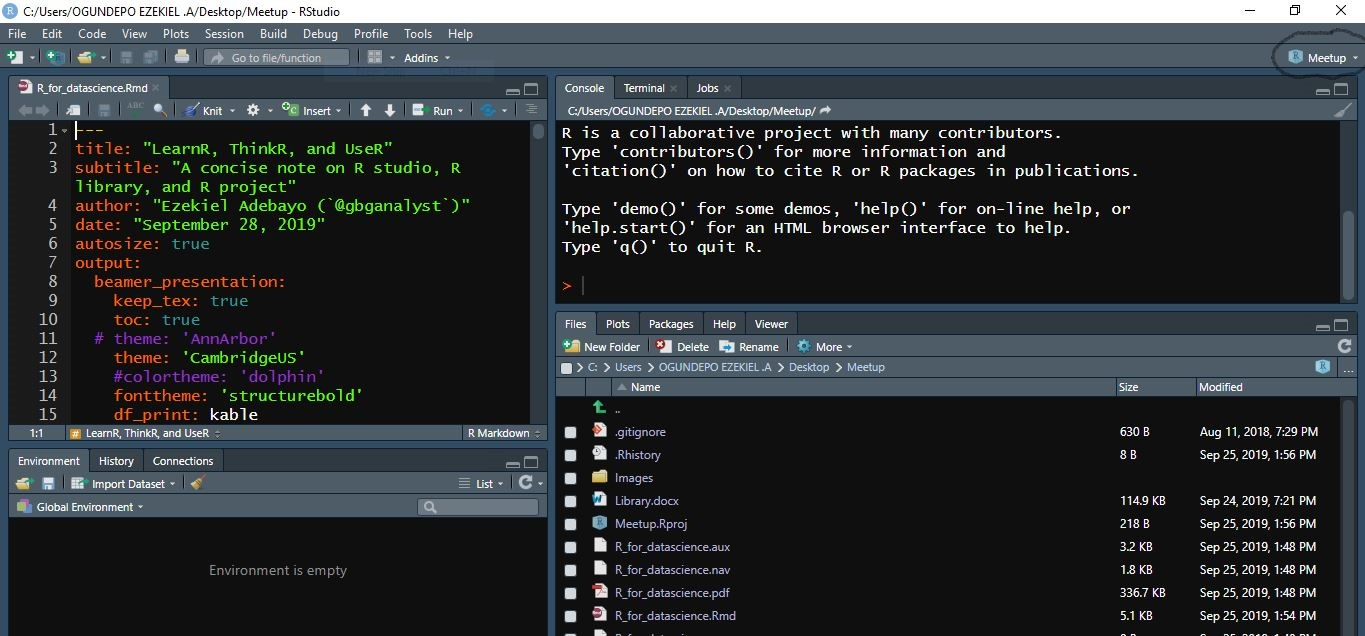
\includegraphics[height=10cm]{Images/step3.JPG}
\caption{RStudio project}
\end{figure}
Hurray! We are in the RStudio project.
\end{frame}

\begin{frame}{}
\protect\hypertarget{section-5}{}

\begin{figure}
\centering
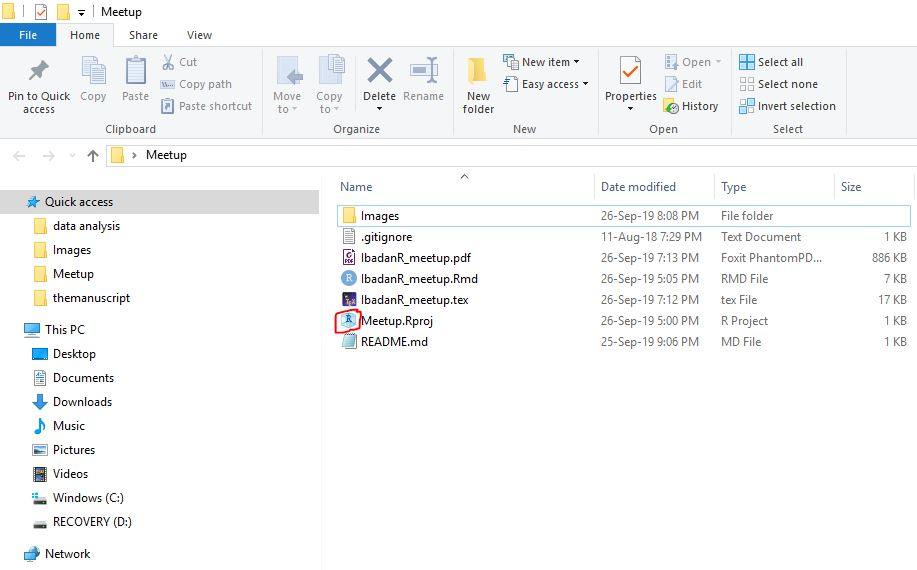
\includegraphics[height=7cm]{Images/step4.JPG}
\caption{Meetup R project directory}
\end{figure}
From now henceforth, you will click \textbf{.Rproj} to open RStudio project.
\end{frame}
\section{Summary}
\begin{frame}{Summary}
\protect\hypertarget{summary}{}

Data science workflow can be done in Rstudio, and we talked about R
packages, how to install them and how to load them. \pause

We also learnt about Rstudio project that enables us to organize our
files i.e.~keep data files, the script, save the outputs and by using
only relative path. \pause

Everything you need is in one place, and cleanly separated from all the
other projects that you are working on.

\end{frame}

\begin{frame}{}
\protect\hypertarget{section-6}{}

\begin{center}
\textbf{Thank you!}
\end{center}

\end{frame}


\begin{frame}{References}
Wickham, H., \& Grolemund, G. (2016). R for data science: import, tidy, transform, visualize, and model data. " O'Reilly Media, Inc.".
\end{frame}

\end{document}
